% options:
% thesis=B bachelor's thesis
% thesis=M master's thesis
% czech thesis in Czech language
% english thesis in English language
% hidelinks remove colour boxes around hyperlinks

\documentclass[thesis=M,english]{FITthesis}[2012/10/20]

\usepackage[utf8]{inputenc} % LaTeX source encoded as UTF-8


\usepackage{graphicx} %graphics files inclusion
% \usepackage{subfig} %subfigures
% \usepackage{amsmath} %advanced maths
% \usepackage{amssymb} %additional math symbols
\usepackage{listings}
\usepackage{color}
\usepackage{caption}
\usepackage{dirtree} %directory tree visualisation

\usepackage{multicol}
\usepackage[section]{placeins}

%% mod colors
\definecolor{titleblue}{rgb}{0.02, 0.37, 0.55}
\definecolor{sectionblue}{rgb}{0.25, 0.44, 0.60}
\definecolor{subsectionblue}{rgb}{0.37, 0.59, 0.77}
\definecolor{gray}{rgb}{0.9,0.9,0.9}

%% mod listings
\DeclareCaptionFont{white}{\color{white}}
\DeclareCaptionFont{black}{\color{black}}
\DeclareCaptionFormat{listing}{\colorbox{gray}{\parbox{\textwidth}{#1#2#3}}}
\captionsetup[lstlisting]{format=listing,labelfont=black,textfont=black}

% % list of acronyms
% \usepackage[acronym,nonumberlist,toc,numberedsection=autolabel]{glossaries}
% \iflanguage{czech}{\renewcommand*{\acronymname}{Seznam pou{\v z}it{\' y}ch zkratek}}{}
% \makeglossaries

% % % % % % % % % % % % % % % % % % % % % % % % % % % % % % 
% EDIT THIS
% % % % % % % % % % % % % % % % % % % % % % % % % % % % % % 

\department{Department of Theoretical Computer Science}
\title{Analysing JavaScript and NPM at scale}
\authorGN{Jakub} %author's given name/names
\authorFN{Žitný} %author's surname
\author{Jakub Žitný} %author's name without academic degrees
\authorWithDegrees{Bc. Jakub Žitný} %author's name with academic degrees
\supervisor{Jan Vitek, M.Sc.}

\acknowledgements{I~am extremely grateful for all guidance, support (material and spiritual) and patience I~received from my supervisor Jan Vitek. I~thank to Petr Maj for pushing the whole project forward when I~was busy, lazy or chaotic and for taking the lead. I~would also like to thank Petr Brzek for understanding my lack of focus and absence at Avocode. My deepest thanks also go to Eva, João, Honza, Ondrej, Michaela and all my friends that supported me during my studies. I~would not finish this without the calming folk tunes of Marhule band either.}

\abstractEN{In this work we looked at different sources of JavaScript code and metadata, collected rich datasets and performed a data analysis on top of them. We have created a pipeline for detecting duplicates within millions of JavaScript files and found that there is more than 90\% of JavaScript files in Github projects that are cloned from somewhere else. We discuss the reasons for the high percentage of clones and present few ideas on what analyses we can to in the future with collected data.
}

\abstractCS{Táto práca skúma JavaScriptové repozitáre a vývojárske metadáta z viacerých zdrojov. Zozbierali sme nieko{\v l}ko datasetov a analyzovali ich základné vlastnosti. Vytvorili sme process na detekciu duplikátov miliónov JavaScriptových súborov a zistili sme, že na GitHube je viac ako 90\% súborov zduplikovaných z iných projektov. Poskytujeme nieko{\v l}ko vysvetlení pre ve{\v l}ké mnošžstvo duplikátov a navrhujeme nieko{\v l}ko ďalších projektov, ktoré by sa zo zozbieranými dátami mohli robiť.}

\placeForDeclarationOfAuthenticity{Prague}
\keywordsCS{big code, github, mining software repositories, ecmascript, javascript, npm, analyza, sourcerercc}
\keywordsEN{big code, github, mining software repositories, ecmascript, javascript, npm, analysis, sourcerercc}
\declarationOfAuthenticityOption{1} %select as appropriate, according to the desired license (integer 1-6)
% \website{http://site.example/thesis} %optional thesis URL


\begin{document}

% \newacronym{CVUT}{{\v C}VUT}{{\v C}esk{\' e} vysok{\' e} u{\v c}en{\' i} technick{\' e} v Praze}
% \newacronym{FIT}{FIT}{Fakulta informa{\v c}n{\' i}ch technologi{\' i}}

\setsecnumdepth{part}
\chapter{Introduction}

Analysing large codebases such as GitHub can provide interesting insights on how programmers use or misuse programming languages, what kind of programming patterns occur in different development ecosystems, and possibly how authors can further improve their languages or runtimes. Looking at software repositories has been in the eyes and minds of researchers at least since mid 2000s \cite{msr_1}. Every year, the analysis of repositories is becoming more complex and today it requires plenty of human and computational resources. Nowadays, we do not only look at the code, its history in version control systems \cite{msr_2} and build artefacts, but we also take into account the libraries and frameworks that code depends on, the activity of developers, and various popularity indicators of files and projects. \\


When analysing such large repositories of code we can use an umbrella term "Big Code" \cite{darpa, jsnice}, similarly as "Big Data" has been used for a general data analyses exceeding certain size or complexity \cite{bigdata}. \\


JavaScript has been rising to the top of programming language popularity indices, such as TIOBE \cite{tiobe_index}, PYPL \cite{pypl_index}, or IEEE Spectrum's ranking. It has gained the current momentum only recently, hence the usage of modern tools like GitHub or StackOverflow is higher, compared to C, Java, or Python programmers. It is therefore not a coincidence that JavaScript is the most popular language on both platforms, according to GitHut statistics \cite{githut} and recent StackOverflow's Developer Survey \cite{so1}. Together with the language, the whole ecosystem has been on the rise. JavaScript is now used to write server-side apps thanks to Node.js, native desktop apps thanks to GitHub's Electron, and also mobile apps thanks to Facebook's React Native or Apache Cordova. Most of JavaScript programmers now use NPM to include the libraries and frameworks into their project, in fact, NPM is the largest of all module repositories out there. According to Modulecounts \cite{modulecounts}, NPM is first with more than twice the modules Maven Central has for Java, Rubygems for Ruby or Packagist has for PHP. \\


Analysing JavaScript source code repositories can have not only interesting results but can also lead to creating useful developer tools \cite{jsnice, darpa}. This work makes first steps in this direction, several datasets with JavaScript code have been created, analysed and the search for clones within them have been performed and discussed.


\section{Structure of the following chapters}

This chapter describes the fundamental motives regarding the purpose and outcome of this work. \\

The next two chapters review academic work and projects that have been dealing with similar problems, as well as examine the required steps that need to be done before we can look at first interesting problems. Chapter 3 covers the structure of datasets for mentioned purposes and the process of data collection. Chapter 4 provides the reader with basic insights  gained from simple dataset analyses. Chapter 5 explores the code duplication that is contained within various repositories in the datasets. \\

Appendices include further methods and results in order to provide better overview of this topic.

\setsecnumdepth{all}
\chapter{Related work}

There has been work somewhat related to the pursuit of better development tools derived from existing code repositories and the Big Code challenge. The Mining Software Repositories conference has been around since 2004 \cite{msr_1} and the first year had already touched this topic \cite{msr_2}. More relevant work has popped up in past few years, especially when GitHub and StackOverflow polished their APIs and started releasing dump archives dedicated to data analysis. \\


Wittern E. et al. look at basic statistics of modules hosted in NPM \cite{js_dynamics}. Authors inspect package descriptions, the dependencies among them, and download metrics, and since NPM packages are usually linked to GitHub source code, they were able to take a look at them as well. In both perspectives, they considered historical data and generated several charts that tell us more about what NPM really stands for. Some of their results are mentioned and built upon in Chapter 4. \\


A~subset of data from GitHub and StackOverflow APIs are also part of publicly available datasets in Google BigQuery. The GitHub part contains repository metadata such as programming languages or licenses, but also the repository contents. BigQuery datasets are publicly available to any logged in user with a Google account. Users can run SQL queries and arbitrary JavaScript code on top of the data. An example of data analysis on top of these datasets is presented in \cite{bq_tabs_vs_spaces}. Authors parsed a billion files from 400000 repositories in 14 programming languages and compared the usage of tabs and spaces for indentation. In results for JavaScript there are 18\% of files that use tabs and the rest is spaces. There are similar analyses discussed in \cite{bq_jshint}, \cite{bq_java_imports}, \cite{bq_angular} and \cite{bq_go}. \\


An example of a tool derived from existing code is JSNice. It is a scalable prediction engine for solving two kinds of problems in the context of JavaScript: predicting (syntactic) names of identifiers and predicting (semantic) type annotations of variables. Experimentally, JSNice predicts correct names for 63\% of name identifiers and its type annotation predictions are correct in 81\% of the cases. In the first week since its release, JSNice was used by more than 30000 developers and in only few months has become a popular tool in the JavaScript developer community \cite{jsnice}. \\


In 2014, the U.S. DARPA agency initiated a program called Mining and Understanding Software Enclaves (MUSE) \cite{muse, darpa} which seeks to make significant advances in the way software is built, debugged, verified, maintained and understood. A~number of projects have presented their progress or have already been published \cite{muse_mit1, muse_mit2, muse_colo}. $Code Phage$ is a system developed for automatic transferring of correct code from donor applications into recipient applications that process the same inputs to successfully eliminate errors in the recipient. Experimental result highlight the ability of CP to transfer code across applications to eliminate out of bounds access, integer overflow, and divide by zero errors \cite{muse_mit1}. $Prophet$ is a patch generation system that works with a set of successful human patches obtained from open-source software repositories to learn a probabilistic, application-independent model of correct code. It generates candidate patches, uses the model to rank the them in order of likely correctness, and validates the ranked patches against a suite of test cases to find correct patches \cite{muse_mit2}.  \\


The following sections describe existing datasets and services that can fall into the "Big Code" category. Some of them became the sources of datasets described in the next chapter.

\section{StackExchange Data Dump}

StackExchange Data Dump is an anonymised dataset of all user-contributed content on the Stack Exchange network. Each site is formatted as a separate archive consisting of compressed XML files. Each site archive includes Posts, Users, Votes, Comments, PostHistory and PostLinks \cite{se_dump}. \\

We are interested in the $Posts.xml$ file from $StackOverflow$ part. The compressed size of the single file is 8,3~GB and it includes over a million JavaScript-related posts. \\

The StackExchange Data Dump is also available at Google's BigQuery. \\

\section{GitHub Archive}

GitHub Archive is a service recording the public GitHub timeline, archiving it, and making it easily accessible for further data analysis \cite{gharchive}. GitHub Archive records all events from the GitHub API \cite{gh_events}, these range from new commits and fork events, to opening new issues, adding new comments and adding new members to a project. All of the events are stored in three datasets by year, month and a day. GitHub Archive datasets are a part of the public datasets on Google's BigQuery. \\

An insight to the data can be obtained by a simple query. The following query counts the number of forked repositories from last year, for example. The result is $9538608$. \\

\lstset{title=Count the number of forks from last year}
\begin{lstlisting}[basicstyle=\small]
SELECT COUNT(*), repo
FROM [githubarchive:year.2016]
WHERE type = 'ForkEvent'
\end{lstlisting}


\section{GHTorrent}

One of the sources for our datasets has been GHTorrent. GHTorrent is an independent copy of the data from GitHub API. It monitors the GitHub public event timeline and for each event it retrieves the content and the dependencies, exhaustively. It then stores the raw JSON responses to a MongoDB database, while also extracting the structure in a MySQL database \cite{ghtorrent}. \\

To access GHTorrent's databases one needs to request access to a SSH tunnel that allows a connection to hosted MongoDB and MySQL instance with the whole dataset. The dataset is also available in Google's BigQuery. \\

The contents of the dataset inside MySQL tables is following. There are 21 tables: 

\begin{multicols}{2}
\begin{itemize}
\item commit\_comments
\item commit\_parents
\item commits
\item followers
\item issue\_comments
\item issue\_events
\item issue\_labels
\item organization\_members
\item project\_commits
\item project\_languages
\item project\_members
\item projects
\item pull\_request\_comments
\item pull\_request\_commits
\item pull\_request\_history
\item pull\_requests
\item repo\_labels
\item users
\item watchers
\end{itemize}
\end{multicols}

The $projects$ table will be one of the sources for our datasets. The last update to the table was performed in September 2016, it contains 33 million row which takes over 5 GB of disk space. There are 10 columns, the most important ones are $id$, $url$ with the link to GitHub API endpoint of given project, $language$ with the main programming language of a repository, and the $forked\_from$ and $deleted$ flags. The former represents the fact whether project had been created as a fork of another existing one or not. The latter is $true$ if the project has been removed from GitHub or its scope has changed from public to private. \\

When connected to GHTorrent's SSH tunnel we can directly query the MySQL database from a client. An insight to the JavaScript-related data can be given by following queries: \\

\lstset{title=Querying GHTorrent for the counts of JavaScript repositories}
\begin{lstlisting}[basicstyle=\small]
SELECT COUNT(id)
FROM projects
WHERE language = 'JavaScript';

SELECT COUNT(id)
FROM projects
WHERE language = 'JavaScript'
AND forked_from IS NULL;

SELECT COUNT(id)
FROM projects
WHERE language = 'JavaScript'
AND forked_from IS NULL
AND deleted = 0;
\end{lstlisting}

The results for the queries are in the order as they were executed $5322424$, $2314083$ and $2011875$. The time GHTorrent database needed to return the first result was $127$ seconds, the next two queries have used the cache and ended in milliseconds. \\

\section{Boa language and infrastructure}

Boa is a domain-specific language and infrastructure that eases mining software repositories. Boa's infrastructure leverages distributed computing techniques to execute queries against hundreds of thousands of software projects very efficiently \cite{boa_web}. The goal of Boa is to ease testing MSR-related hypotheses. The authors came up with it when trying to generally solve a problem with them at a very large scale, at a fine-grained level of detail, and with full history information. \cite{boa_intro}

\lstset{title=Counting projects in a specific language}
\begin{lstlisting}[basicstyle=\tiny]
p: Project = input;
js_count: output sum of int;

foreach (i: int; match(`^javascript$`, lowercase(p.programming_languages[i])))
    jsc_count << 1;
\end{lstlisting}

\lstset{title=The output of Boa job 50839}
\begin{lstlisting}[basicstyle=\tiny]
cofeescrpit_count[] = 203531
js_count[] = 1473096
typescript_count[] = 8105
\end{lstlisting}

The job is publicly available at \url{https://goo.gl/yatpvZ}. \\

Boa offers huge comfort for Big Code analysers and already contains both metadata and actual source code in their datasets. Currently they only provide outdated datasets of limited size. The size and richness of Boa datasets is similar to the public ones on Google BigQuery, however, users can not upload their own. The latest Boa dataset from GitHub is from September 2015. Boa is also not nearly as fast as BigQuery. \\

\begin{center}
\begin{figure}[h!]
	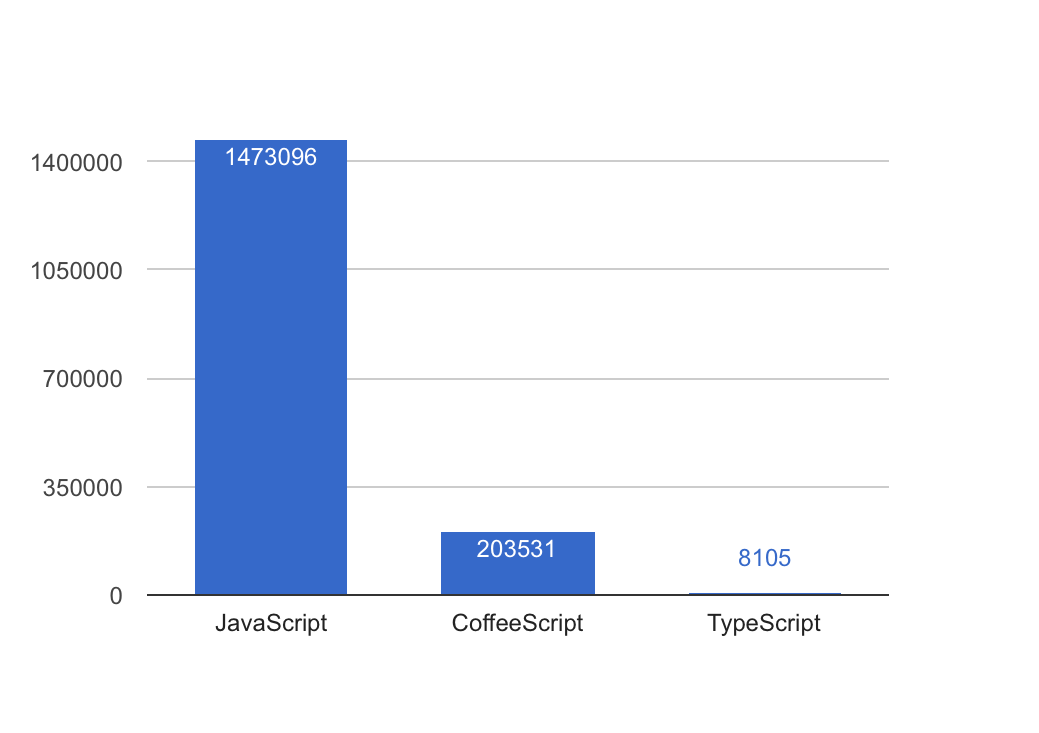
\includegraphics[totalheight=265pt]{images/boa_counts.png}
	\caption{JavaScript, CoffeeScript and TypeScript  project counts in Boa's 2015 September/GitHub dataset}
	\label{fig: boa_counts}
\end{figure}
\end{center}


\section{npms.io}

The npms continuously analyzes the NPM ecosystem, gathering as much information as possible from a variety of sources, including GitHub, David and Node Security Platform (NSP). Using the collected information, a final score for each package is calculated based on four different aspects: quality, maintenance, popularity and personalities. \cite{npms}. Users can use NPMS instead of official \url{https://npmjs.com} to search for NPM modules and learn more about the estimated quality of each one of them.


\chapter{Analysis of the problem}

In order to follow our goals we need to create a dataset that better suits our needs. It would be even better if we could create a data infrastructure that is extendable and as up-to-date as possible. \\

The previous chapter has mentioned the GitHub API and projects built on top of it. These are a great start. However, if we want to utilize the full potential of GitHub we have to connect the metadata from the API to the actual source code content of Git repositories that are hosted on GitHub. Furthermore, we should also add metadata from NPM API to the dataset as it contains different popularity indicators than GitHub. These are not always correlated. GitHub API provides developer activity events and number of stars, forks and contributors for each project. NPM API has numbers of downloads for each module. All interesting parts of both APIs will be mentioned in the next chapter. \\

Besides enriching the actual code with different kinds of available metadata, we would like to be able to regenerate our dataset as often as possible. Since GitHub API is limited we cannot call it too often \cite{gh_limits}. This is where the GHTorrent and GitHub Archive are useful. They can give us necessary dumps for every event and we can recreate the picture of data at GitHub without really using our limits for API calls. \\

In the following sections we are presenting a few possible directions one can take when the foundations of such infrastructure are laid. \\

\section{Asserting the quality of dependencies}

Can we determine whether JavaScript library or framework is safe to use? How active is the library we include in our project and is it likely to die in following months or years? What are the quality metrics determining the robustness of a library or module? These are the questions JavaScript developers ask when looking for a module dependency that will be included in their project. There is no JavaScript standard library and even for the smallest things JavaScript programmers tend to depend on an open-source project from NPM or GitHub. We can look at the dataset and expect some of the features to be strong quality indicators. Among them we see the number of stars, forks, subscribers or number of downloads per year, month, and per week. Besides these, we can look at the size of projects, their dependencies, number of maintainers and contributors, issues and whether there are tests or readme files available. \\

NPMS is one attempt for such assertion. Their formula considers more than 25 quality indicators and calculates a quality score for each NPM module. The quality indicators have been manually chosen to reflect the best practices of JavaScript developers \cite{npms_arch}. Figure 2.1 shows the whole pipeline of how NPMS observes the changes on NPM, collects the data and evaluates the score. \\

\begin{center}
\begin{figure}[h!]
	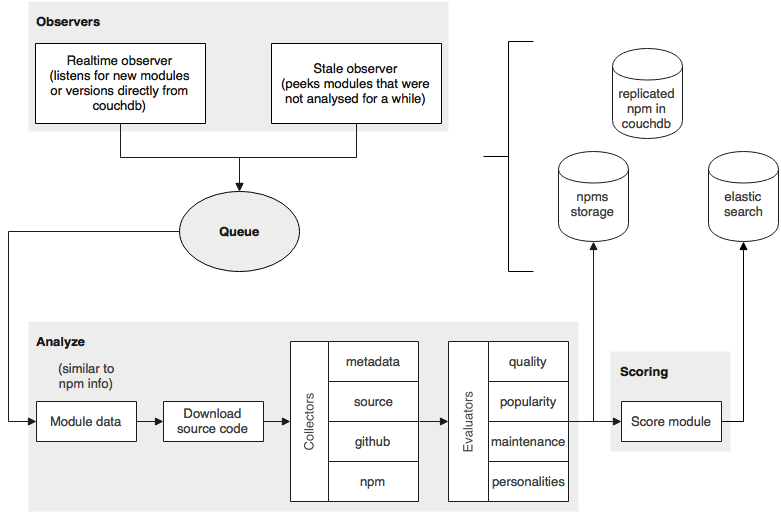
\includegraphics[totalheight=225pt]{images/npms_analysis.png}
	\caption{The NPMS architecture}
	\label{fig: npms_analysis}
\end{figure}
\end{center}


The NPMS approach is very popular and more and more developers use it to search for the right dependencies. However, we don't see it scalable and robust enough. What if the quality indicators change over time? How do we properly balance their value? Could we try training a regression model to calculate a quality score? Would it be possible to get better results than NPMS? Will the size of our dataset be enough for such a complex model? It is definitely worth a try, but creating the right training dataset will be the main challenge. One scenario would be choosing a single ultimate quality indicator, such as GitHub stars or NPM download counts, and trying to learn this from the data as a quality score. Another possibility could be reinforcement learning where the reward would be  calculated from the quality score. \\

The challenge of learning the quality of NPM modules or GitHub projects in general can be reduced to subproblems. We can try to create a classifier for determining the quality of Readme files on GitHub. Readme file content and the list of files in root directory are shown on the default page for each project on GitHub. Readme files contain several quality indicators that NPMS uses in their calculations. Classifying these could be a good subproblem to solve.

\section{Searching for clones}

Another take on the dataset we will have is clone analysis. Once we have such a large and rich dataset of repositories it is interesting to know how can we reduce its size. How many repositories are exact clones of one another? How many repositories are forks of one another? And how many files are copied within and across the repositories? This will help us understand not only the redundancy in the dataset but also the behaviour of the developers and how they are used to the fact that JavaScript now has a module manager \cite{npm}. \\

There is a difference between repositories that are forks and repositories that are exact clones of one another. A fork is a copy of a repository that is stored on GitHub (or other Git hosting service) under different namespace \cite{gh_forks}. We can determine whether a repository is a fork using GitHub API or we can employ our own algorithm for this.  Forked repositories have common history up to certain point but their latest form can be completely diverged and there might be very few common files. An example of such case is when Google forked WebKit's WebCore component and separated the development of new features that were customised for Chrome \cite{blink}. Another example is $io.js$, the Node.js fork that had planned to develop separate project under an "open governance model", but let itself back into the Node.js upstream. \cite{iojs, iojs2, iojs3}. Exact clones in our case are repositories that have all files in common. This might be the result of one being a fork of another without any further work being done, it might also be that a programmer manually copied all files to a new project and committed them separately. \\

We expect cloned files to have different causes. That is why we will do a qualitative analysis of a random sample to see what these might be. \\

\section{Searching for occurrences of StackOverflow snippets}

If we manage to set up the whole pipeline for detecting clones, we could use it to search for occurrences of StackOverflow snippets. We have already mentioned the StackExchange Data Dump in Chapter 1. We can use the contents of $Posts$ and $Answers$ from the dataset to create a dataset of JavaScript snippets and search for the clones of these on GitHub.

\section{Enhancing the infrastructure}

As we mentioned earlier, we intend to put forward the whole infrastructure for analysing JavaScript repositories. The infrastructure should be scalable and extendable. Newly calculated data should be reusable for further analyses and new data from the APIs should be available as soon as possible. This will make it even more robust than NPMS. \\

In addition to the observers, collectors, evaluators and the databases that NPMS has, we propose adding an additional layer of API that will enable users to upload new or derived data. This could work in a similar way that BigQuery offers. \\

\begin{center}
\begin{figure}[h!]
	\hspace*{0.5cm}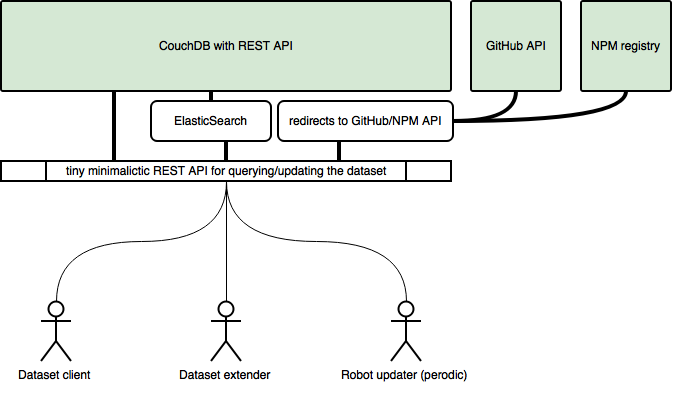
\includegraphics[totalheight=205pt]{images/npms_alt.png}
	\caption{Proposal for NPMS enhancement}
	\label{fig: npm_counts}
\end{figure}
\end{center}


\section{Proposed data analyses}

We have mentioned four possible directions we can take to follow our goal. Due to time constrains, it is not possible to implement all of them within the scope of this work. We will start with creating the datasets, we will implement an analysis to get to know the basic properties of the data and we will create the pipeline for clone detection within the data.

\chapter{The data}

The data we intend to use come from several sources. The two main ones are

\begin{enumerate}
\item JavaScript Git repositories from GitHub with whole Git history and GitHub metadata
\item metadata from NPM API \cite{npm}.
\end{enumerate}

None of these are currently in a format that we consider appropriate for analyses we want, however, we do help our case with the already pre-processed dataset from GHTorrent that we can access without limits \cite{ghtorrent}. \\

Besides these, we will also be putting together a dataset of StackOverflow JavaScript snippets. This dataset will consist of JavaScript code from StackOverflow questions and answers, enriched with metadata from StackExchange API \cite{so_api}. \\

As we will be using SourcererCC \cite{scc_1} clone detector for detecting clones, we have connected all the sources into a single dataset, similar to the one that authors used for their cause. In their dataset, there is a Git bare repository for working with code history and Git metadata, latest snapshot of the code from Git, usually master branch, GitHub metadata in a special folder and also NPM metadata in another special folder. This enables us to connect the results from various sources and possibly use the historical data from Git too. \\

Note that Git metadata are different than GitHub metadata. The former represents the metadata from Git itself, such as commit messages, dates of contributions, names of branches, etc., and the latter consists of the data taken from GitHub API \cite{gh_api} where we can see for example the number of project’s issues, pull requests, stars or contributors. \\

We have created several sub-datasets so we can work faster on smaller scale and so that we see the results on the most popular projects separately without distortion from small or non-maintained projects. There is an extreme amount of JavaScript projects on GitHub. In fact, together with repository forks there are over $5$ million of them. At NPM there are over $300000$ projects and more than 90\% of them are linked to their GitHub code. These numbers will be discussed thoroughly in Chapter 4. \\

We created five datasets as follows.

\begin{enumerate}
\item $top1000$ - consists of the most starred 1000 GitHub projects written in JavaScript,
\item $70k$ - consists of randomly picked 70000 GitHub projects written in JavaScript
\item $1M$ - consists of 1 million randomly picked JavaScript GitHub projects that are not forks
\item the $NPM$ dataset - NPM project metadata from the NPM API
\item the $StackOverflow$ JavaScript code snippets
\end{enumerate}

\begin{table}[]
\centering
\begin{tabular}{@{}cccccccc@{}}
\toprule

Data & Projects & Files & Collection time & \\ \midrule
top1000  & 1000  & 84433 & hours  & \\
70k  & 72325  & 18940371  & days &  \\
1M  & 916082 & 41652400 & weeks & \\
\bottomrule
\end{tabular}
\caption{Overview of datasets}
\label{gh_meta_popularity}
\end{table}

We have collected the datasets in two batches. In the beginning, our goal was to collect the first two datasets only, the $70k$ being the main one. We did not have a good estimate of the size it will take neither the time we will need. \\

For generating the $top1000$ dataset we only needed the GitHub API. The $/search$ endpoint is limited to exactly 1000 results \cite{gh_search}. We can specify a language we want the results to be in and also the sorting criterion. In this case we want top 1000 JavaScript projects sorted by popularity. One of the popularity indicators on GitHub is the number of $stars$. A~$curl$ request for getting these looks like this: \\

\lstset{title=Curl request for top1000 project from GitHub API}
\begin{lstlisting}[basicstyle=\tiny]
curl -ni \
"https://api.github.com/search/repositories?sort=stars&q=language:JavaScript"
\end{lstlisting}

We present detailed description of the GitHub API endpoints we use in the following section. \\

\section{GitHub API and its quotas}

GitHub API is REST API that returns JSON payloads. We can query it with $curl$ command line application or with any HTTP client from any programming language. The API endpoints that we are interested in are \\

\begin{itemize}
\item \textbf{/search} 
\item \textbf{/repos/:owner/:repo} or $repo$ for short
\item \textbf{/repos/:owner/:repo/commits} or $commits$ for short
\end{itemize}

We will be querying the $repo$ and $commits$ endpoints to get meta information about the repositories. Especially the popularity indicators — stargazer, fork and subscriber counts, but also available dates, and commit counts. \\

Shortened responses for $repos/jakubzitny/big.js$ look as follows. The important parts we will be analysing in this work are emphasized. \\

\lstset{title=GitHub API response from /repos/jakubzitny/big.js endpoint}
\begin{lstlisting}[basicstyle=\tiny]
 {
   "id": 48099297,
   "name": "big.js",
   "full_name": "jakubzitny/big.js",
   "owner": { ... },
   "private": false,
   "html_url": "https://github.com/jakubzitny/big.js",
   "description": "Big.js",
   "fork": false,
   "url": "https://api.github.com/repos/jakubzitny/big.js",
   "created_at": "2015-12-16T09:06:13Z",
   "updated_at": "2016-01-21T16:46:35Z",
   "pushed_at": "2016-07-31T09:48:38Z",
   "git_url": "git://github.com/jakubzitny/big.js.git",
   "ssh_url": "git@github.com:jakubzitny/big.js.git",
   "clone_url": "https://github.com/jakubzitny/big.js.git",
   "size": 8,
   "stargazers_count": 0,
   "language": "CoffeeScript",
   "forks_count": 0,
   "default_branch": "master",
   "subscribers_count": 0,
   ...
 }
\end{lstlisting}

\newpage

\lstset{title=GitHub API response from /repos/jakubzitny/big.js/comits endpoint}
\begin{lstlisting}[basicstyle=\tiny]
[
  {
    "sha": "5c87c7e503eae82fd8636189c28a60eaadb5d452",
    "commit": {
      "author": { ... },
      "committer": { ... },
      "message": "add basic crawling in MUSE format",
      "tree": { ... },
      "comment_count": 0
    },
    "author": { ... },
    "committer": { ... },
    "parents": [ ... ]
  },
  ...
]
\end{lstlisting}

The limitation when querying the GitHub API is $5000$ requests per hour for authenticated user \cite{gh_limits}. This scales to $70000$ or more repositories with a difficulty. We would need 14 hours to get only the basic metadata from one endpoint for each repository. \\

We also want to get count of all commits for a repository from GitHub API. To do this, we have to look into the HTTP headers of the response from $commits$ endpoint. The $commits$ endpoint returns the list of commits from the newest one on pages by 30 commits. The $Link$ header contains a link to the $next$ and $last$ page. Let us define the number of pages as $pages$, and the number of commits on the last page as $lp$. \\

The total number of commits $n$ equals to

$$
n = (pages - 1) * 30 + lp
$$

For getting this information from the GitHub API we need to issue two separate requests. If we want to save the extra request and we do not need the exact $n$, we can create an upper bound $n'$ that is equal to

$$
n' = pages * 30
$$.

When the whole repository clone is available, one can also use the $git$ CLI application to get the exact $n$. \\

\lstset{title=Git CLI command to count commits in a repository}
\begin{lstlisting}[basicstyle=\small]
git rev-list --all --count
\end{lstlisting}

\section{Git repository contents}

Besides the meta information from GitHub API we are also cloning the contents of the default branch in the Git repository. We have the Git URL from the API and for simple analysis we need only the latest version of it. We use the $git$ CLI client directly with $--depth 1$ argument. To clone contents of the repository from the examples above we will need the following: \\

\lstset{title=Git CLI command to get latest repository without history}
\begin{lstlisting}[basicstyle=\small]
git clone --depth 1 https://github.com/jakubzitny/big.js.git
\end{lstlisting}


\section{NPM API}

Figure \ref{fig: npm_counts} shows the exponential growth of modules published on NPM. According to \cite{modulecounts}, NPM grows by almost 340 new packages every day. There has been little work done on top of the NPM API though. It does not have any documentation and the only official client is the $npm$ CLI application. In Chapter 1 we have mentioned four projects and one publication \cite{js_dynamics} that did analysis on top of NPM API. Most of them are focusing on visualisation of the NPM package versions \cite{npm_by_numbers}, download counts \cite{npm_stats, npm_stat, js_dynamics} and dependency relationships \cite{js_dynamics, npm_discover}. \\

\begin{center}
\begin{figure}[h!]
	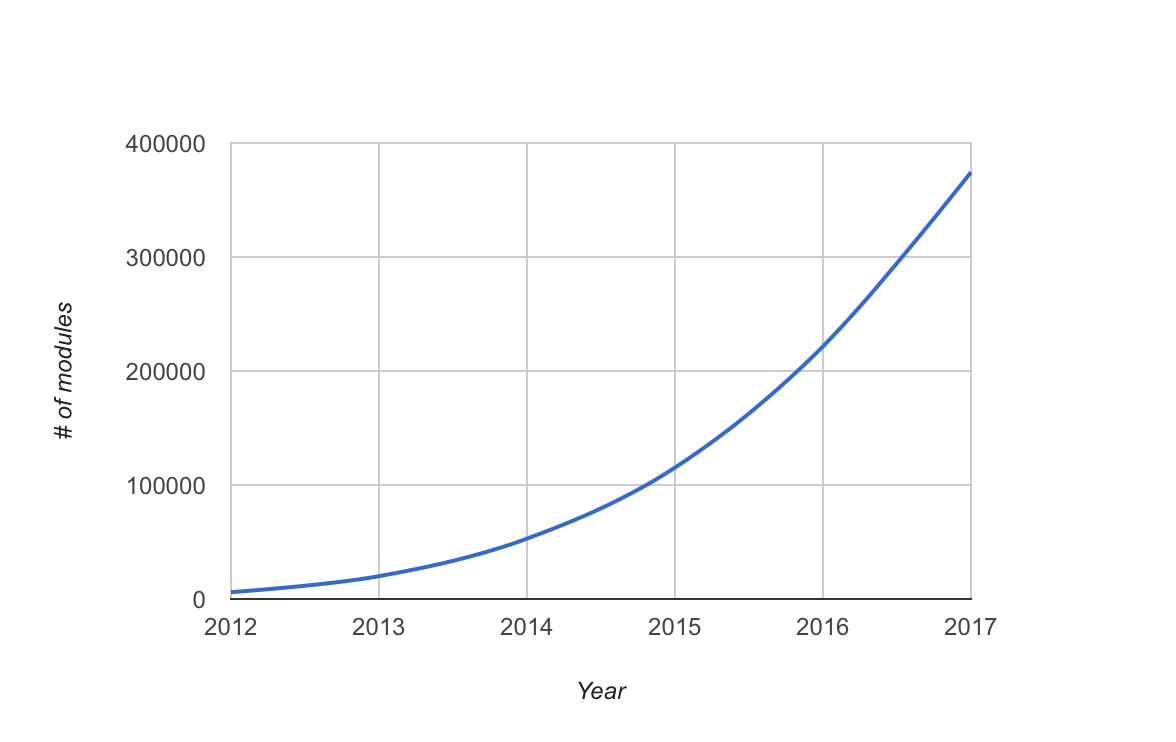
\includegraphics[totalheight=225pt]{images/npm_counts.png}
	\caption{The growth of NPM modules}
	\label{fig: npm_counts}
\end{figure}
\end{center}

By documenting the API, generating the dataset and examining it we hope to provide better insight into what kind of content NPM really hosts. \\

We had to look into the source code of the NPM CLI application to see the API endpoints it requests \cite{npm_gh_api}. There are two APIs available at \url{https://registry.npmjs.org} and at \url{https://skimdb.npmjs.com}. The former includes all data that NPM CLI app uses, the latter is a CouchDB with module metadata \cite{npm_arch}. \\

The endpoint for a single module metadata is \textbf{/:name/:version/}. Shortened response to $GET$ request to \url{https://registry.npmjs.org/react/latest} returns following. \\

\lstset{title=NPM API response with module metadata}
\begin{lstlisting}[basicstyle=\tiny]
{   
  "_id": "react@15.4.2",
  "_nodeVersion": "6.3.1",
  "_shasum": "41f7991b26185392ba9bae96c8889e7e018397ef",
  "name": "react",
  "description": "React is a JavaScript library for building user interfaces.",
  "version": "15.4.2",
  "main": "react.js",
  "dependencies": { ... },
  "bugs": { ... },
  "directories": { ... },
  "dist": { ...  },
  "engines": { ... },
  "files": [ ... ],
  "homepage": "https://facebook.github.io/react/",
  "keywords": [ "react" ],
  "license": "BSD-3-Clause",
  "maintainers": [... ],
  "repository": {
      "type": "git",
      "url": "git+https://github.com/facebook/react.git"
  },
  "scripts": { ... },
  ...
}
\end{lstlisting}


There is a lot of interesting information from the $package.json$ file of the module \cite{npm_packagejson} and additional internal NPM keys with $\_$ prefix such as $\_id$, $\_nodeVersion$, $\_resolved$, $\_shasum$, $\_npmOperationalInternal$, or $\_npmUser$. \\

The CouchDB metadata uses the default CouchDB REST API for querying \cite{couchdb_api}. So, one can use the \textbf{/\_all\_docs} endpoint to look for all available packages and the \textbf{/registry/:name} to look for all versions of a module. There is also another special API endpoint at \url{https://registry.npmjs.org} which is used by the NPM CLI app when searching and caching the registry. It is \textbf{/-/all} and it returns an array of metadata for all packages at once. We will be using this response as the source of our NPM dataset. \\

\section{Code}

All of the datasets we mentioned above and used in this thesis are available at \url{https://github.com/jakubzitny/big.js}. 

\chapter{Basic data analysis}

In this chapter we are focusing on datasets we have created. We are gathering insights and exploring interesting properties of the data. We look at the code statistics in the first part, the GitHub metadata in the second part and the NPM metadata at the end.

\section{JavaScript on GitHub}

We present the properties of the GitHub 70k and 1M datasets in this section. We chose to start working on a smaller scale so that we get a glimpse of the data, fix bugs, and make the platform more stable. \\

\begin{center}
\begin{figure}[h!]
	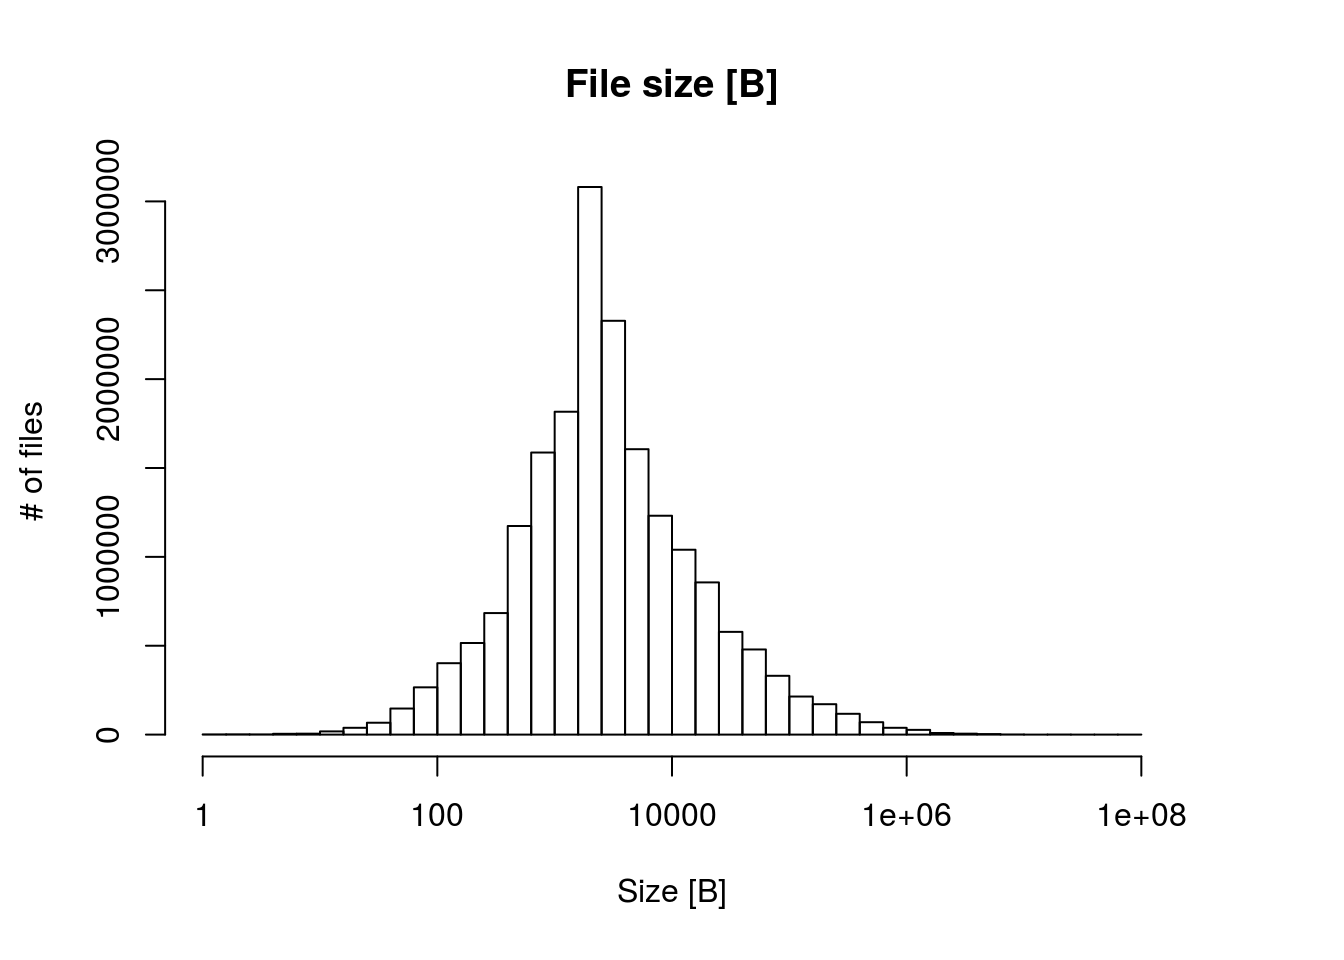
\includegraphics[trim=0cm 0cm 2cm 0cm, totalheight=230pt]{images/70k_bytes.png}
	\caption{Distribution of file sizes in the $70k$ dataset}
	\label{fig: 70k_bytes}
\end{figure}
\end{center}

First we look at the general file statistics. What kind of JavaScript files do we have in our dataset? How big the files are? During the tokenization we have been collecting the line counts and the sizes for each file. Figure 4.1 shows the distribution of file sizes in the $70k$ dataset. Median value is $2,4~kB$ per file and mean is $20,3~kB$. The largest file in this dataset is over $90~MB$ large and it is available from \cite{largest}. \\

Figure 4.2 shows the distribution of lines of code (LOC) per file among all files in the $70k$ dataset. We have surprisingly large number of one-liners, the reasons will be discussed in following sections. Median value is 41 lines, mean is 422.2 and the longest file in terms of lines of code is almost 2.8 million lines long. The file is available from \cite{longest}. The difference between the mean and median shows that there is a lot of extremely big or long files. \\

\begin{center}
\begin{figure}[h!]
	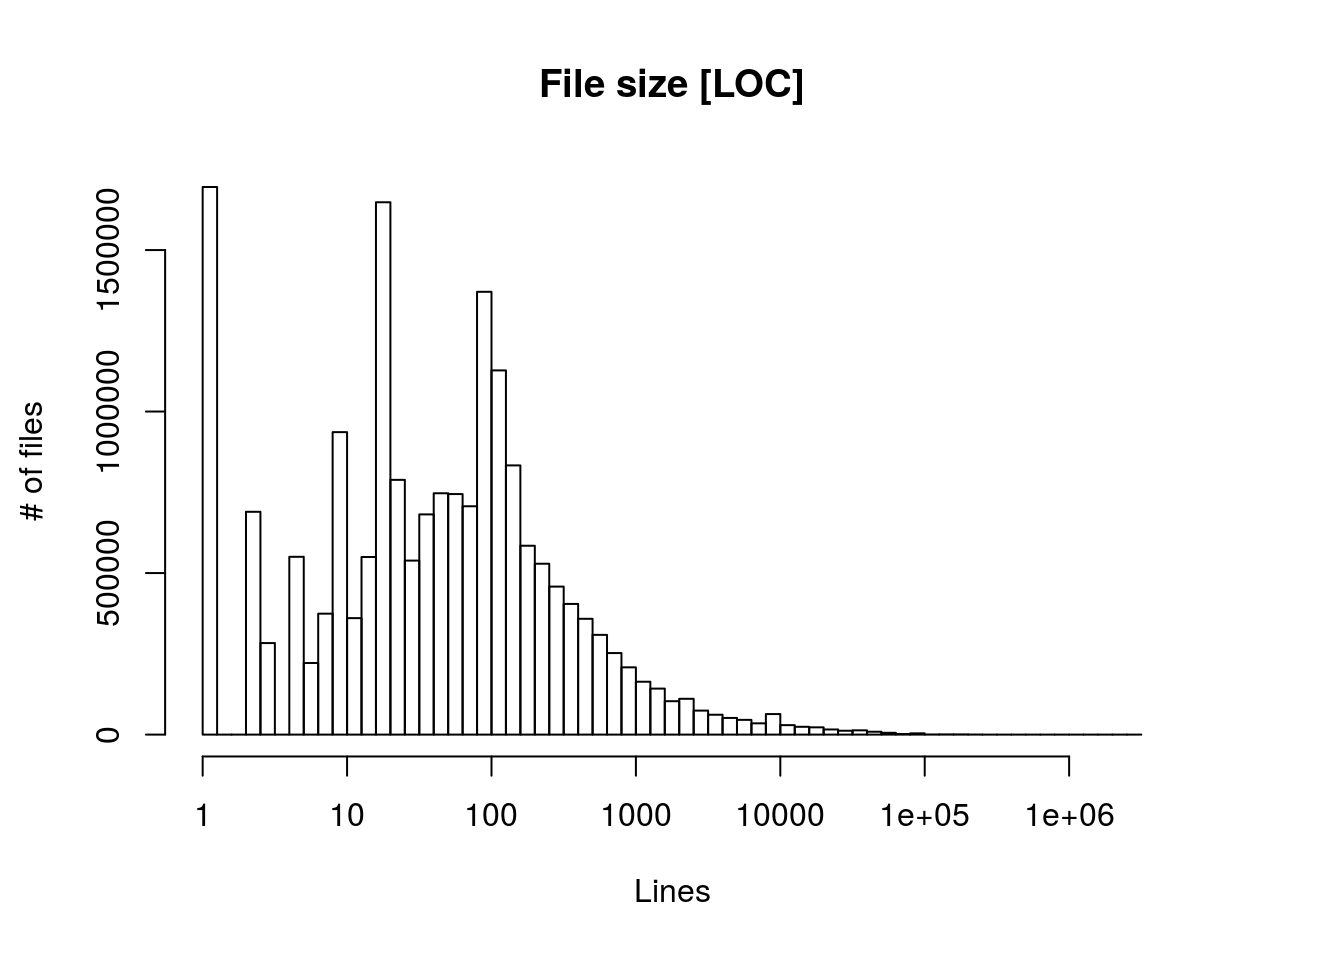
\includegraphics[trim=0cm 0cm 2cm 0cm, totalheight=230pt]{images/70k_locs.png}
	\caption{Distribution of LOC per file among all files in the $70k$ dataset}
	\label{fig: 70k_locs}
\end{figure}
\end{center}


Figures 4.3 and 4.4 show the distribution of token counts in a file. The first sums all the tokens together and the second one counts only the unique tokens to capture the diversity of them. Median number of tokens in a file in the $70k$ dataset is 177 and the median of unique tokens is 83. \\

\begin{center}
\begin{figure}[h!]
	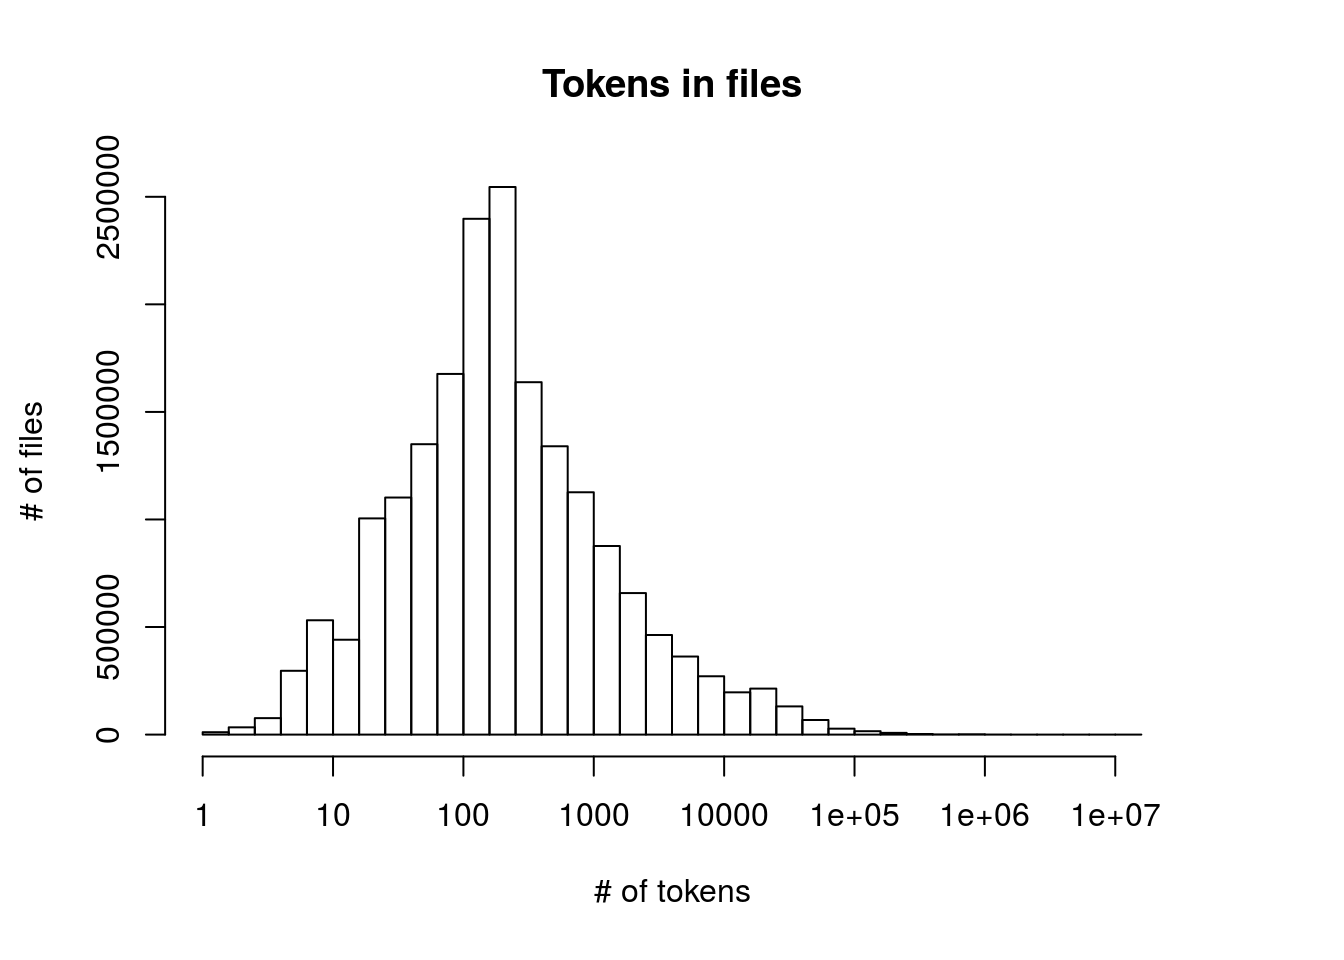
\includegraphics[totalheight=230pt]{images/70k_tokens.png}
	\caption{Distribution of token counts in a file in the $70k$ dataset}
	\label{fig: 70k_tokens}
\end{figure}
\begin{figure}[h!]
	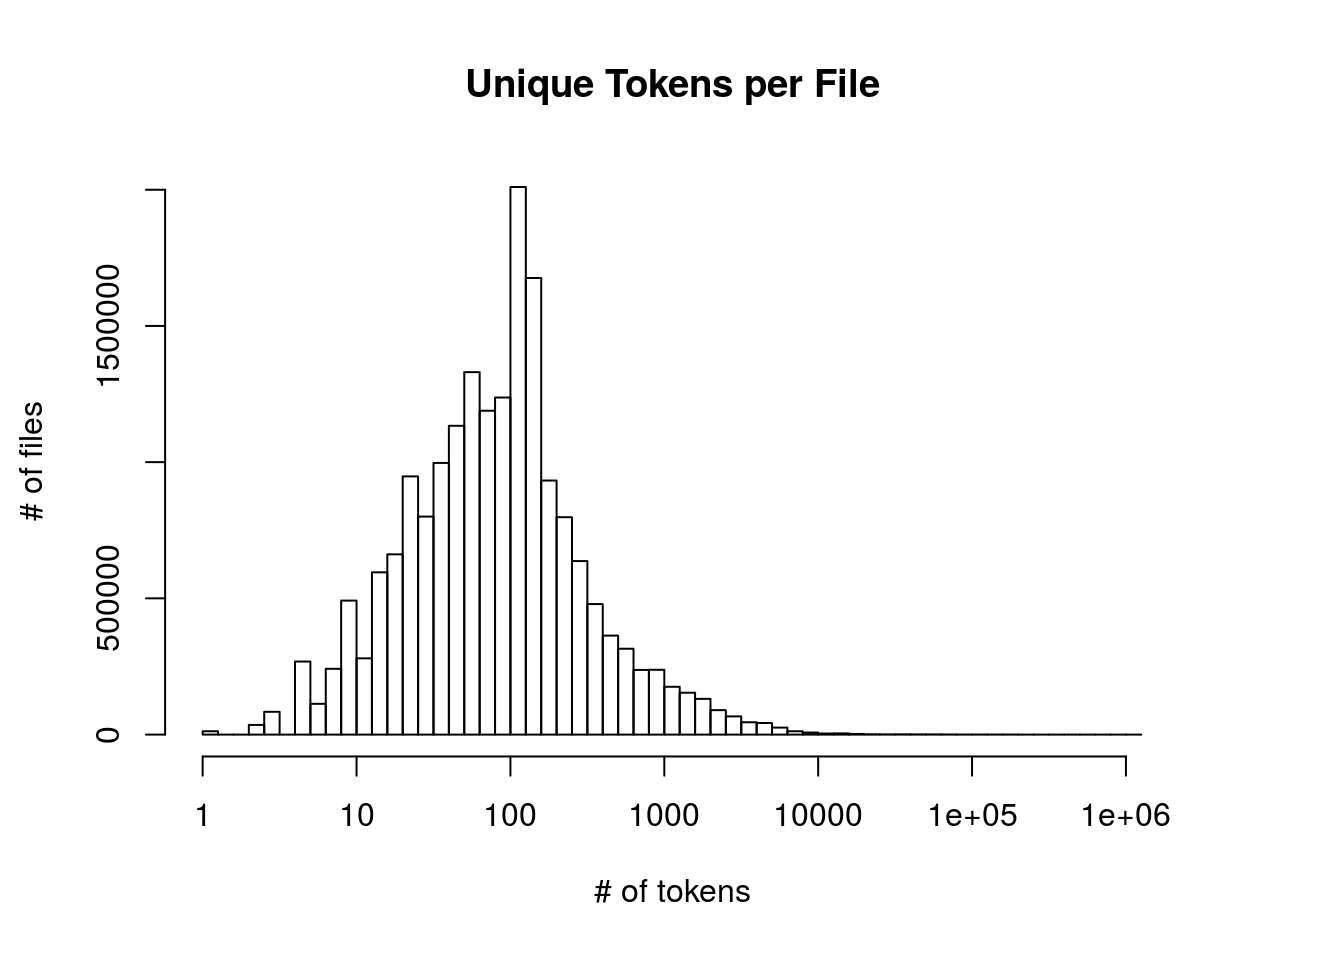
\includegraphics[totalheight=230pt]{images/70k_uniquetokens.png}
	\caption{Distribution of unique token counts in a file in the $70k$ dataset}
	\label{fig: 70k_uniquetokens}
\end{figure}
\end{center}

Besides the line counts and the sizes for each file, our tokenizer also kept track of the white spaces and comments. We can compare how many percent of the file contents are actually code and how many is only white spaces and comments. On average, there is 6\% of the JavaScript file comments and 14\% white spaces in the $70k$ dataset. \\

On Figure 4.5, we can see that most of the files have less than 10\% of the comments per file.

\begin{center}
\begin{figure}[h!]
	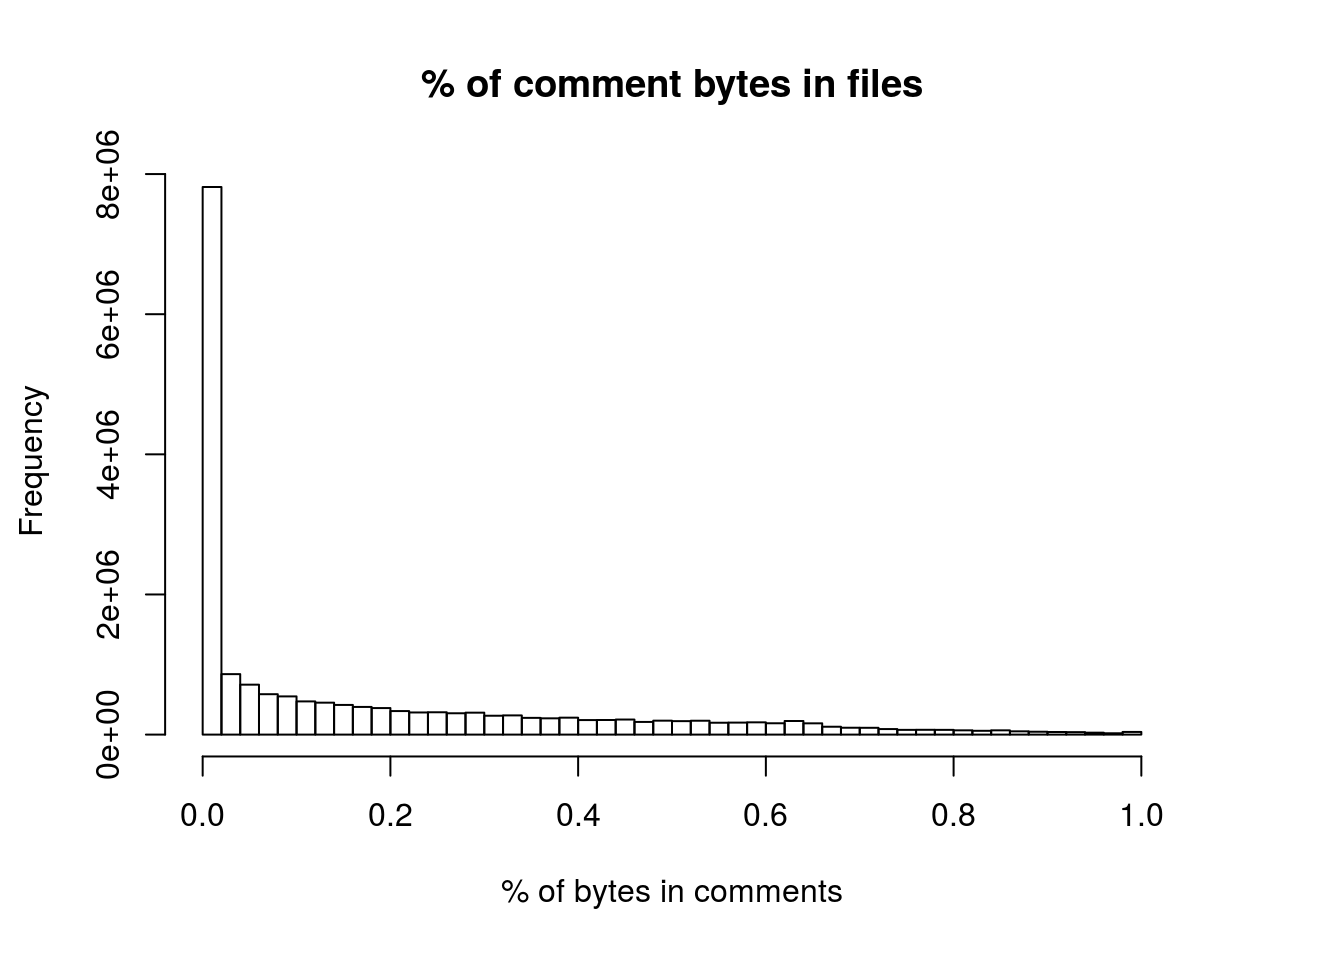
\includegraphics[totalheight=230pt]{images/70k_comments.png}
	\caption{Distribution of whitespace bytes in a file in the $70k$ dataset}
	\label{fig: 70k_comments}
\end{figure}
\end{center}


To see how projects look compared to each other, we will look at the project-level insights. Figure 4.4 shows the distribution of file counts in our $70k$ dataset. We can see that most of the projects have $1$ to $10$ files. The median is $15$, the mean is $261.9$ and the maximum is $409000$ files. Almost half a million files is quite a lot for a single project. We will investigate it further in this chapter. \\

\begin{center}
\begin{figure}[h!]
	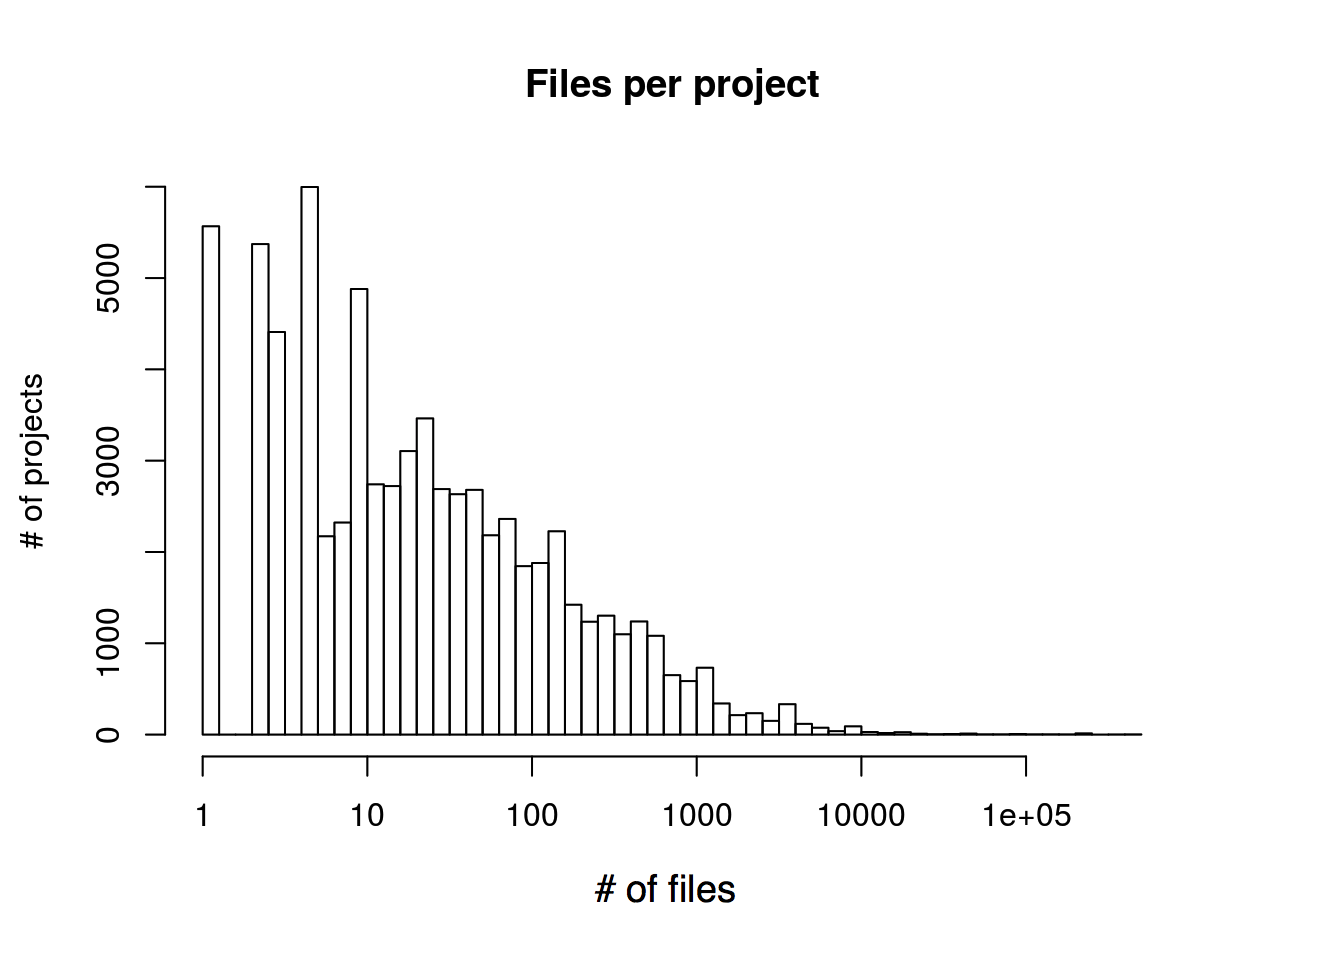
\includegraphics[totalheight=270pt]{images/70k_filespp.png}
	\caption{Distribution of file counts per project}
	\label{fig: 70k_filespp}
\end{figure}
\end{center}


After looking at the numbers and cherry-picking projects that contain large or a lot of files we have decided not to include forks in the larger scale. This should be the first step in reducing the numbers of duplicated files. We have also identified a few other possible sources of duplication in the datasets. For instance, people often commit minified and obfuscated versions of JavaScript client libraries into their repositories. Even worse case is when commits contain the whole working directory with the complete tree of dependencies from NPM or Bower. \\

When we scaled up from the $70k$ to $1M$ dataset we found similar statistics for file sizes and counts in projects. There were no forked repositories and we still found large number of duplicates and extremely large number of files in some projects. The results of duplicate detection are detailed in Chapter 5. We will discuss the large projects here. \\

When we inspected the largest projects we found out that a lot of them contain $node\_modules$ directory. This is a place where $npm$ stores the dependencies, however, this should not be committed into Git repository. It takes too much space and it is not a source-code that programmers want to change or track \cite{gitignore}. If programmers need to lock a specific version of dependencies into the code, there are special mechanisms for that, there is no need to commit libraries or frameworks into the version control \cite{shrinkwrap, yarnlock}. \\

It turns out that there is 70\% of files in our dataset that are contained within $node\_modules$ directory. These 70\% of the files are located only in 5\% of the projects we have in the $1M$ dataset. There is also 2\% of files that are inside $bower\_components$ directory which is managed by alternative Bower module manager for JavaScript. And there is over 10\% of minified files inside the whole dataset. Minified JavaScript files are concatenated and sometimes also obfuscated libraries or arbitrary code that is served to client browsers as one big file so it does not have to do a lot of separate requests for assets to a server. Minified files usually have $.min.js$ extension. \\

We have looked at the most popular Node modules and minified files among these. Table 4.1 shows the list of top 5 Node module names. The most common module in this particular subset of NPM programs is $lodash$. Incidentally, it is also one of the most popular NPM modules all together \cite{npm}.

\begin{table}[h]
\centering
\begin{tabular}{@{}cccc@{}}
name & count & percentage of files &    \\ \midrule
lodash & 14668258 & 35\% &\\
core-js & 10856121 &  26\% &\\
es5-ext & 3211456 & 7,7\%  &\\
mout & 2074284 & 5\% &\\
babel-runtime & 1920365 & 4,6\% &\\
\bottomrule
\end{tabular}
\caption{Most common module names contained in $node\_modules$}
\label{node_modules}
\end{table}

Table 4.2 shows the list of top 10 files with $.min.js$ extensions. Programmers used to commit $.min.js$ libraries into repository when building simple client applications in the past. The most popular minified libraries here are jQuery and Bootstrap which are the prototype client-side libraries that many developers use and love.

\begin{table}[h]
\centering
\begin{tabular}{@{}ccccc@{}}
name & count & percentage of min.js files & percentage of files overall &   \\ \midrule
jquery & 1226486  & 28\%   & 3\% &\\
bootstrap & 312156  & 7\% & 1\% &\\
angular &  290421 & 7\% & 1\%&\\
kendo & 225967 & 5\% & 1-\% &\\
lodash & 142141  & 3\% & 1-\% &\\
underscore & 109292 & 3\%& 1-\% &\\
rx & 54717  &  1\%& 1-\% &\\
ionic &  50838 &  1\%& 1-\% &\\
moment & 35639  & 1\% & 1-\% &\\
respond & 31461  &  1\% & 1-\% &\\
\bottomrule
\end{tabular}
\caption{Most common $.min.js$ files}
\label{minified_files}
\end{table}

\newpage

We looked at the versions of jQuery programmers are using. In our case the committed $.min.js$ files are either named $jquery.min.js$ or there is a version included in the filename. $jquery-1.9.1.min.js$ for example. jQuery follows the Semantic Versioning of packages. This means every new release of a library has three numbers, major, minor, and patch. $1.9.1$ for example. Approximately 50\% of jQuery occurrences have versions included. \\

Figure 4.6 shows the distribution of the patch versions in our $1M$ dataset. The most used $patch$ version here is $1.9.1$, followed by $1.7.1$ and $1.8.2$. If we merge the patch version counts, $1.8$ and $2.1$ will be the most popular. Regarding major versions the first one takes 71,8\%.

\begin{center}
\begin{figure}[ht]
	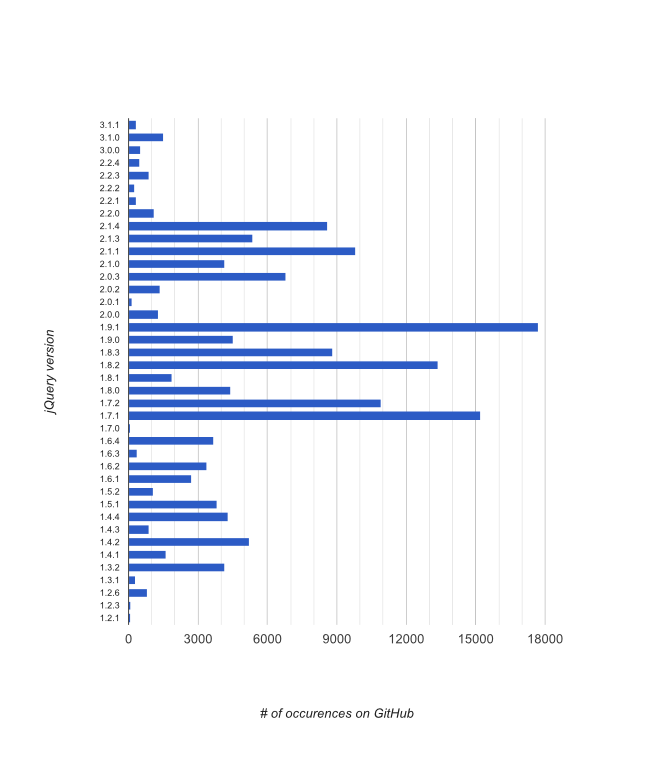
\includegraphics[trim=4cm 0cm 3cm 2.5cm, totalheight=530pt]{images/jquery_nm_patch.png}
	\caption{Distribution of jQuery patch versions in $.min.js$ files in $1M$ dataset}
	\label{fig: jquery_nm_patch}
\end{figure}
\end{center}

\section{Popularity on GitHub}

The popularity on GitHub has three main indicators:

\begin{enumerate}
\item stars
\item watchers (or subscribers)
\item forks
\end{enumerate}

Starring is a feature that lets users bookmark repositories. $Stars$ are shown next to repositories to show an approximate level of interest. Stars have no effect on notifications or the activity feed \cite{gh_starring}. Users can also $watch$ a project. Watching a Repository registers the user to receive notifications on new discussions, as well as events in the user's activity feed \cite{gh_watching}.  Forks are usually connected with contributions to projects. New contributors usually fork main project to their namespace, make local changes and then submit a Pull Request to the upstream.

\begin{center}
\begin{figure}[ht]
	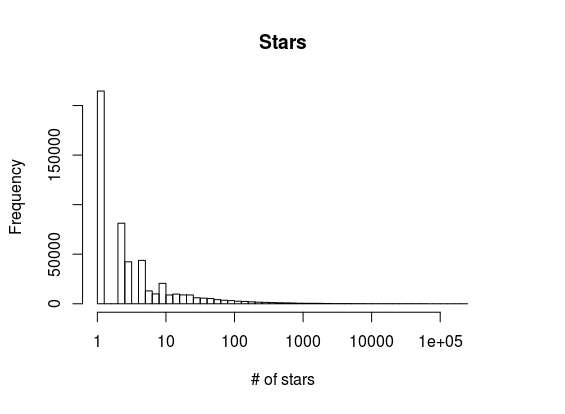
\includegraphics[totalheight=270pt]{images/meta_stars.png}
	\caption{Distribution of the number of stars in projects}
	\label{fig: meta_stars}
\end{figure}
\end{center}

\begin{center}
\begin{figure}[h!]
	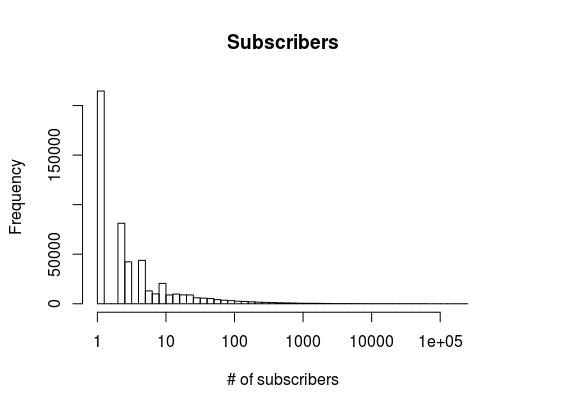
\includegraphics[totalheight=270pt]{images/meta_subs.png}
	\caption{Distribution of the number of subscribers in projects}
	\label{fig: meta_subs}
\end{figure}
\end{center}

We can see that most of the projects have 0 stars, 0 forks and 0 watchers. This is natural for such a big hosting service as GitHub is. There is many personal projects, that might not be active anymore or are not used by many people, maybe small companies, at schools, etc. There is a fair amount of  open-source libraries that are used a lot. The link between the NPM users and GitHub repositories is mentioned in the next section.

\begin{table}[h!]
\centering
\begin{tabular}{@{}cccccccc@{}}
& Min & Q1 & Med & Mean & Q3 & Max &     \\ \midrule
Stars  & 0.00  & 0.00 & 0.00   & 8.81 & 1.00 &  210925.00 &\\
Forks  & 0.00   & 0.00  & 0.00 & 2.06 & 0.00 & 26776.00 & \\
Watchers  & 0.00  & 1.00 & 1.00   & 2.42 & 1.00 & 5690.00 & \\
\bottomrule
\end{tabular}
\caption{Summary of stats for star, watch and fork counts}
\label{gh_meta_popularity}
\end{table}


Results presented in this section are results for the whole set of 2 million non-forked JavaScript GitHub repositories that are listen in GHTorrent's project table. Stars are not present in the GHTorrent dataset so we had to use our scripts from the third chapter to generate these. \\

The maximum number of both stars and subscribers in a JavaScript project goes to FreeCodeCamp \cite{fcc}, maximum number of forks has Angular.js \cite{gh_angular}.

\begin{center}
\begin{figure}[ht]
	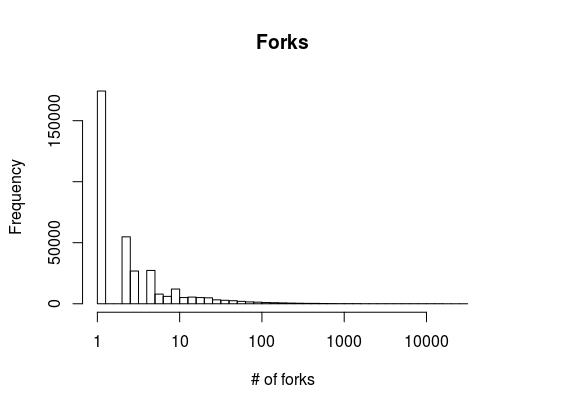
\includegraphics[totalheight=240pt]{images/meta_forks.png}
	\caption{Distribution of the number of forks in projects}
	\label{fig: meta_forks}
\end{figure}
\end{center}

\begin{center}
\begin{figure}[h!]
	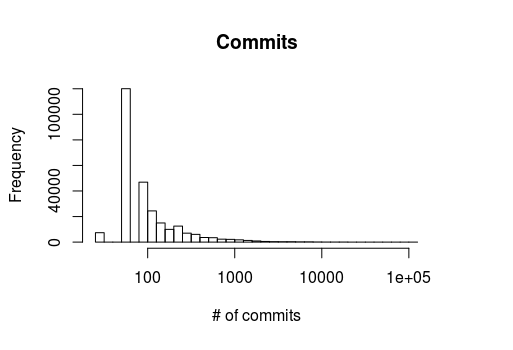
\includegraphics[totalheight=240pt]{images/meta_commits.png}
	\caption{Distribution of the number of commits in projects}
	\label{fig: meta_subs}
\end{figure}
\end{center}

\newpage

\section{NPM}

Figure below shows the exponential growth of modules published on NPM. In this section we are analysing the NPM dataset that is described in previous Chapter. NPM grows by almost 340 new packages every day \cite{modulecounts}. \\



One of the ways to start a NPM project is to use the $npm init$ command. The NPM CLI then asks developer to enter the following information, which is saved in the $package.json$ file at the root level of the repository:

\begin{multicols}{2}
\begin{itemize}
\item name
\item version
\item description
\item entry point
\item test command
\item git repository
\item keywords
\item license
\end{itemize}
\end{multicols}

The name, version, description, repository info, keywords and license are also present in our dataset.


\subsection{Git and version control systems}

We have found that 82\% of modules have the $repository$ field present in their $package.json$ files. Out of these, 99\% have type Git. It is understandable that this number is so high as NPM command line application specifically asks developers to enter Git repositories. In the missing 1\% there are a few SVN, Mercurial and Bazaar repositories. 98\% of the Git repositories resolve to endpoints at GitHub, 0.8\% to BitBucket and 0.5\% to GitLab.

\begin{center}
\begin{figure}[h!]
	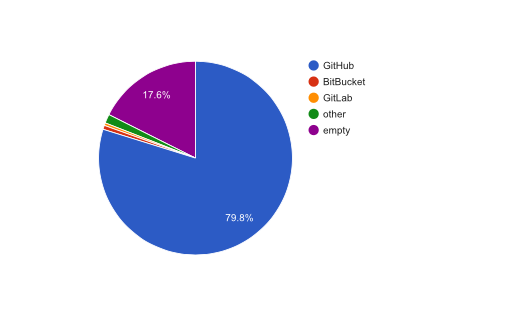
\includegraphics[totalheight=265pt]{images/npm_gits.png}
	\caption{The share of Git hosting services in NPM modules}
	\label{fig: npm_gits}
\end{figure}
\end{center}

\subsection{Licenses}

79\% of the modules have the $License$ field filled out. The NPM command line application uses the ISC license automatically, however, the most used license is MIT, followed by ISC, Apache, BSD family, and GPL-like licenses. \\

97\% of Apache licenses are Apache 2.0. \\

32\% of the BSD family occurrences is 3-clause license under names "revised", "new", or "modified", 30\% is 2-clause license also known as "simplified", or "FreeBSD License" and 38\% of the cases it is not specified whether authors desire BSD-3-Clause or BSD-2-Clause. Only 9 modules explicitly ask for the original 4-clause BSD License. \\

57\% of the GPL-like licenses link the latest GPLv3 license \cite{license_gpl}, 17.5\% are GPLv2 \cite{license_gpl2} and 1\% goes to both LGPLv3  and AGPLv3 \cite{license_lgpl3, license_agpl3}, while old LGPLs and AGPLs are almost not used at all \cite{license_lgpl20, license_lgpl21, license_agpl1, license_agpl2}. \\


\begin{center}
\begin{figure}[h!]
	\hspace*{-1cm}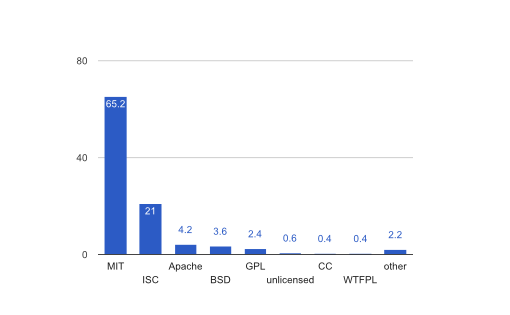
\includegraphics[totalheight=265pt]{images/npm_licenses.png}
	\caption{The share of open-source licenses in NPM modules}
	\label{fig: npm_licenses}
\end{figure}
\end{center}

The rest of the modules include Creative Commons licenses \cite{license_ccs}, other custom or modified licenses or deliberately "unlicensed" modules. Worthy of mention is also WTFPL license with a 0.4\% share \cite{license_wtfpl}. \\

\begin{center}
\begin{figure}[h!]
	\hspace*{-1cm}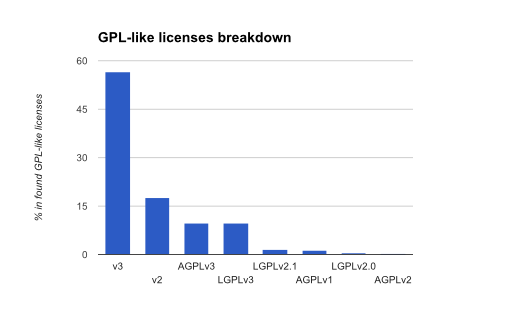
\includegraphics[totalheight=265pt]{images/npm_licenses_gpl.png}
	\caption{The share of GPL licenses among all GNU GPL derivatives}
	\label{fig: npm_licenses_gpl}
\end{figure}
\end{center}

GitHub released the statistics of overall License usage across all programming languages and revealed that the MIT License had 44,69\%, GPL-likes 23\%, and BSD family had 6\%. The most popular among BSD licenses had been version 2 \cite{gh_licenses_share}. \\

\subsection{Descriptions}

95\% of all modules have non-empty description in metadata. The average length of description is 7.7 words per description and  the mean is 6. After removing the stop words the 10 most popular words in the corpus of all descriptions are:

\begin{multicols}{2}
\begin{enumerate}
\item node
\item simple
\item plugin
\item module
\item library
\item javascript
\item api
\item your
\item react
\item package
\end{enumerate}
\end{multicols}

We can see that almost all of the words have somewhat general meaning. It is either a synonym to "module" — "plugin", "library", or "package" or it is related to the platform ("node", "javascript"). The only instance of a specific library is "react" \cite{react_gh}. \\

\subsection{Keywords}

We have checked the most used keywords in all modules. 69\% of modules have non-empty keyword array in metadata and surprisingly "react" is the most used one.

\begin{multicols}{2}
\begin{enumerate}
\item react
\item api
\item javascript
\item css
\item node
\item gruntplugin
\item json
\item yeoman-generator
\item cli
\item plugin
\item express
\item angular
\item react-component
\item test
\item gulp
\item html
\item browser
\item ember-addon
\item framework
\item http
\end{enumerate}
\end{multicols}


Front-end developers often compare increasingly popular frameworks React, Angular and Ember. In this simple statistic, in over 350000 modules, there is 24952 modules with "react", 9095 with "angular" and 3690 with "ember" keyword occurrences. React already attracted our attention in previous section. \\

Another interesting comparison might be the number of keywords with $grunt$ and $gulp$ occurrences. These are runners that a lot of JavaScript project use for building, testing, installing and other configuration tasks. Both of can be used as Make or CMake in the C/C++ world \cite{js_make}. JavaScript developers often compare these as well \cite{gruntgulp}. Right now the NPM contains 8619 modules in which keywords match $.*grunt.*$ regular expression. There is 8752 gulp matches.


\subsection{Readme files}

The statistics for Readme file metadata are straightforward. Most of the projects on NPM, similarly as on GitHub are initialized with a Readme.md file. This file is also displayed on module's default page. Markdown with extension ".md" is the preferred markup language. For historical reasons, there are also several text, RST and ADOC Readme files.

\begin{center}
\begin{figure}[h!]
	\hspace*{-1cm}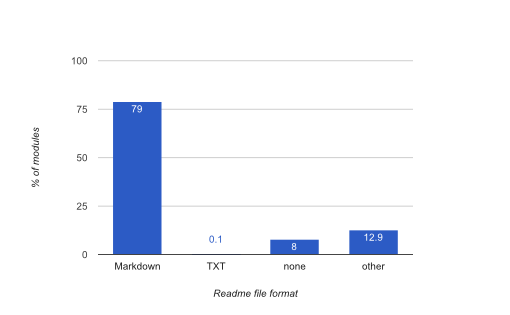
\includegraphics[totalheight=265pt]{images/npm_readmes.png}
	\caption{The share of formats of Readme files in NPM modules}
	\label{fig: npm_readmes}
\end{figure}
\end{center}

\subsection{Analysis code}

The code we used for calculating the numbers and generating the charts is available at

\begin{itemize}
\item \url{https://github.com/jakubzitny/big.js}
\item \url{https://github.com/reactorlabs/js-reports}
\end{itemize}

\chapter{Clone detection}

There are three different types of clones we want to look for: $file-hash$, $token-hash$ and $sourcerer-cc$ clones. Two files that are $file-hash$ clones have equal MD5 hash. That means that they are exact copies of one another. $Token-hash$ clones have the same MD5 hash of a $token$-$count$ pairs string which captures changes in comments and whitespaces. $Sourcerer-cc$ clones are files reported by SourcererCC clone detector with a 70\% threshold. Following sections give details about SourcererCC and the $token$-$count$ pairs. \\

Incidentally, we can define inverse labels for different types of unique files: $file-hash$ unique file will be a file that is not a $file-hash$ clone. It goes similarly for $token-hash$ and $sourcerer-cc$ uniques. \\

\section{SourcererCC}

\cite{scc_pre} and \cite{scc_1} present efficient clone-detection mechanism and application called SourcererCC. Instead of understanding the whole programming language, SourcererCC calculates the occurrences of tokens in a file, stores them in inverted index and uses it to quickly search for clones. It finds clones where amount of duplicates is above a defined range, 70\% for example. This means we can still detect files with whitespaces and comments added, removed, or some variable names and strings changed. And since we are not analysing the syntax or semantics of the source code we can do this very fast and scale the clone detection to Big Code. The clone detection can be performed in different levels of granularity. We can compare files, functions or blocks. For the purpose of this work we will only work with files. \\

Authors released the source code of SourcererCC at GitHub \cite{scc_gh}. The main part — the $clone-detector$ — is written in Java. The input to the $clone-detector$ is preprocessed version of files we want to compare. The preprocessed version is generated by a tokenizer. A~sample tokenizer that works for various programming languages is provided in the source code, it is written in Python. For several reasons we have implemented two different tokenizers for the JavaScript dataset. We will describe them later in this chapter. \\

Once we have our datasets, the preprocessing consists of splitting each source file by separators to a string of $token$-$count$ pairs. Separators vary from one programming language to another. For JavaScript the separators are operators and whitespaces. The unique id of a file together with $token$-$count$ pairs are written as a one-line string into a file that is fed into $clone-detector$. \\

\lstset{title=Example code in Java}
\begin{lstlisting}[basicstyle=\tiny]
/**
 * Execute all nestedTasks.
 */
public void execute() throws BuildException {
  if (fileset == null || fileset.getDir(getProject()) == null) {
    throw new BuildException("Fileset was not configured");
  }
  for (Enumeration e = nestedTasks.elements(); e.hasMoreElements();) {
    Task nestedTask = (Task) e.nextElement();
    nestedTask.perform();
  }
  nestedEcho.reconfigure();
  nestedEcho.perform();
}
\end{lstlisting}

\lstset{title=Example output of a tokenizer for Java code, breaklines=true}
\begin{lstlisting}[basicstyle=\tiny]
2,1,@#@for@@::@@1,"Fileset@@::@@1,perform@@::@@2,was@@::@@1,configured"@@::@@1,throw@@::@@1,if@@::@@1,elements@@::@@1,null@@::@@2,nextElement@@::@@1,nestedTask@@::@@2,execute@@::@@1,e@@::@@3,nestedTasks@@::@@1,throws@@::@@1,getDir@@::@@1,void@@::@@1,Enumeration@@::@@1,nestedEcho@@::@@2,not@@::@@1,new@@::@@1,getProject@@::@@1,fileset@@::@@2,hasMoreElements@@::@@1,Task@@::@@2,public@@::@@1,reconfigure@@::@@1,BuildException@@::@@2
\end{lstlisting}


There are three types of separators here:

\begin{enumerate}
\item $@\#@$ - occurs only once, splits the unique fileId and the contents
\item $,$ - splits each $token$-$count$ pair
\item  $@@::@@$ - splits tokens from the token count
\end{enumerate}

\subsection{Custom tokenizers}

Since we plan to continue with detection of clones on lower levels of granularity in the future, sooner or later we will need a custom tokenizer that understands JavaScript. The notion of a block is different in JavaScript and Python, for example. \\  Another reason for implementing our own tokenizer is that our initial testing of the SourcererCC code with Python tokenizer exposed some problems. One of the main ones was performance of tokenizing minified JavaScript files that are present in our datasets. Exact numbers and details on these were mentioned in previous chapter. \\

We have developed and tested a JavaScript tokenizer that is built on top of Esprima library \cite{lib_esprima}. This tokenizer is available on GitHub at \cite{gh_tokenizer_source} and has already been offered to the authors of SourcererCC for adding it to their official repository. \\

After detecting clones on the small $top1000$ dataset we have found out that scaling it to hundreds of thousands or million projects will not be feasible. \\

We decided to rewrite the tokenizer one more time in $C$, collect the data on the fly and detect $file-hash$ and $token-hash$ clones by the tokenizer already. This way the tokenizer will be even faster and large chunk of the dataset will be filtered out after the first preprocessing. We call this the $reactor$ tokenizer, its implementation was not part of this work so the detailed description is available in appendix. We have used this tokenizer to run clone detection on top of the two largest datasets (1M and 2M). \\

\section{Clone detection pipeline}
We have our datasets from Chapter 3 and we do preprocessing with a tokenizer. During this phase, the tokenizer generates various information as side effects of file tokenization. We capture numbers of

\begin{itemize}
\item tokens
\item unique tokens
\item lines and bytes of code
\item lines and bytes of comment code
\item whitespace lines and bytes
\end{itemize}

After writing the statistics on the side, the main output of the tokenizer goes to SourcererCC. SourcererCC reports clone groups that it has found. We load the results into the database and analyze.


\section{Results}

The first iteration of our clone detection was run with our custom JS tokenizer on the $top1000$ dataset. The results showed that there over 90\% of cloned files with 70\% threshold. The $70k$ dataset had even higher number of clones. \\

We explain the high number of clones in the $70k$ dataset by having the forked repositories in it. We have not filtered the forks from the GHTorrent source and we chose random 70000 projects from all 5008554 projects there. Since there is 45\% of projects that are cloned and additional 11\% are moved, deleted or made private since the GHTorrent snapshot was taken, there is over 50\% chance of project being a fork there. Chapter two explains this dataset and the numbers more thoroughly. After the $70k$ analysis we have decided to remove forks in $1M$ and $2M$ datasets.\\

When exploring the largest project clones we found out that many of them were forks of a $cdnjs$ repository that stores tens of thousands JavaScript libraries. The original repository is available at \url{https://github.com/cdnjs/cdnjs} and the project still works as a CDN for front-end development at \url{https://cdnjs.com}. \\

After cherry-picking some files from the clone groups in results from the $70k$ dataset we have found that the most cloned file — $is-implemented.js$ — occurs in $11346$ files spread across $114$ projects. Now, there is already an emerging pattern. The file, and it is not only the most cloned file, but several others as well, occur in the same project multiple times. This should not happen in a project. And if so, it should not happen at this scale — so many times and in so many different projects. After we had gathered results for the 1M dataset we noticed that there is a large amount of library code from NPM contained directly in a lot of repositories. We did not notice this right after analysing the $70k$ results. There is one more indication that this was happening and it is the average and median number of files in a project. On average there was supposed to be $261,9$ files inside a project while the median was only 15. \\

We have collected the results for the 1M dataset as well. This was done on different machines and we have fully utilised the Reactor tokenizer. In over 41 billion files spread across almost 1 million JavaScript projects we found 6.79\% file-hash unique files, 5.86\% token-hash unique files and 4.46\% files that have less than 70\% similarity in tokens with other files. \\

\begin{table}[]
\centering
\begin{tabular}{@{}cccccccc@{}}
\toprule

Data & Projects & Files & File-equals & Hash-equals & SCC- equals & \\ \midrule
top1000  & 1000  & 84433 & 86\%   & 87.5\% & 90\% &\\
70k  & 72325   & 18940371  & 90,5\% & 91,9\% & 95.2\% & \\
1M  & 916082  & 41652400 &  93.2 & 94.1 & 95.5 & \\
\bottomrule
\end{tabular}
\caption{Final clone-detection results for $top1000$, $70k$ and $1M$ datasets}
\label{gh_meta_popularity}
\end{table}

There are several reasons why the cloning is so high in our datasets. First and foremost, there is large amount of people that commit the library or framework dependencies right into their Git repository. This is discouraged in the JavaScript community and very likely in others as well. This leads to a presence of $node\_modules$ or $bower\_components$ directories in the roots of a lot of repositories. To be exact, this amounts to over 70\% of the files in our $1M$ dataset. The reasons why this is the cause of such a high number of clones will be explained in following subsection. Another share of the $file-hash$ clones is contained in copied minified library files that are also committed directly into the repositories.\\



\subsection{Hardware}

The whole $top1000$ analysis took us 36 hours with a tokenizer that was not optimized for heavy loads yet. The analysis was run on a quad-core laptop with 16GB of RAM. \\

The tokenization of the $70k$ dataset took us one day and the SourcererCC clone detection ran for four days on an Amazon machine with 64GB of RAM and 16 CPU cores. \\

The tokenization of the 1M dataset ran on a desktop PC with 32 GB of RAM and 3TB of disk. It took us 15 days. The SourcererCC part was run on even larger machine with 112 CPU cores and 252GB of memory and we needed 3 days for this to finish. \\

\setsecnumdepth{part}
\chapter{Conclusion}

We have collected a number of new datasets for analysing the JavaScript and NPM ecosystem — a dataset with top 1000 most starred JavaScript repositories from GitHub together with its metadata, dataset with random 70000 projects from GitHub that is good for testing analyses and getting a glimpse of the data that is present on GitHub, and finally a dataset with 1 million projects with their metadata.

We have calculated surprising code duplication across the whole GitHub. 95\% of the JavaScript files on GitHub have a clone somewhere else. The reasons for such a high number of clones are mostly developers' unfamiliarity with Git or the module ecosystem. They tend to copy and commit a lot of libraries and frameworks directly into the source-code version control systems. This is discouraged in most of the module managers for other programming languages and it is discouraged in JavaScript as well \cite{gitignore}. \\

This work has been part of a wider research focused on GitHub's code duplicates. The authors of SourcererCC \cite{scc_1} are building on their previous work expanding the clone detection for C/C++, Java, and Python ecosystems. Some of the datasets we have created will be used in Darpa's MUSE program \cite{muse}. This work is also a part of JavaScript initiative within Programming Research Laboratory at CTU with long-term goal of improving JavaScript tooling and runtime by understanding JavaScript BigCode. \\

In the future we will collect the clone detection results for all JavaScript projects on GitHub and compare them with C/C++, Java, and Python results. We also plan to look deeper into history of Git repositories and search for more complex properties of the clones. We are already gathering results for occurrences of snippets from our StackOverflow dataset in JavaScript files from GitHub. We have described the StackOverflow dataset in Chapter 3. Our future work also includes the unfulfilled proposals from Chapter 2: asserting the quality of JavaScript modules and enhancing the whole infrastructure for "live" analysis. Eventually we will be trying to accept or reject the hypothesis that machine learning might enable new opportunities in the area of program analysis for development, security or runtime performance enhancements in a similar way that \cite{jsnice, muse_mit1, muse_mit2, muse_colo} do.

\bibliographystyle{iso690}
\bibliography{mybibliographyfile}

\setsecnumdepth{all}
\appendix

\chapter{Acronyms}
% \printglossaries
\begin{description}
\item[AGPL] Affero General Public License
\item[API] Application Programming Interface
\item[CC] Creative Commons
\item[CDN] Content Delivery Network
\item[CLI] Command Line Interface
\item[FAC] Frequently Applied Change
\item[GPL] General Public License
\item[LGPL] Lesser General Public License
\item[LOC] Lines of Code
\item[MIT] MIT License, originating at the Massachusetts Institute of Technology
\item[MSR] International Conference on Mining Software Repositories
\item[MUSE] Mining and Understanding Software Enclaves
\item[NPM] Node Package Manager
\item[NSP] Node Security Platform
\item[VCS] Version Control System
\end{description}


\chapter{Contents of enclosed CD}

%change appropriately

\begin{figure}
	\dirtree{%
		.1 readme.txt\DTcomment{the file with CD contents description}.
		.1 src\DTcomment{the directory of source codes}.
		.2 big.js\DTcomment{implementation scripts}.
		.2 SourcererCC\DTcomment{SourcererCC sources with our tokenizers}.
		.2 js-reports\DTcomment{R scripts for generating summaries and charts}.
		.2 thesis\DTcomment{the directory of \LaTeX{} source codes of the thesis}.
		.1 text\DTcomment{the thesis text directory}.
		.2 thesis.pdf\DTcomment{the thesis text in PDF format}.
	}
\end{figure}

\end{document}
